\chapter{Administrativia}

\section{Getting \vcsnv}
The version \VcsnVersion\xspace of the \vcsn platform can be downloaded
from \\
\code{http://www.lrde.epita.fr/cgi-bin/twiki/view/Vaucanson/Vaucanson\VcsnVersion}

Other previous versions of the \vcsn platform can be downloaded
from \\
\code{http://vaucanson.lrde.epita.fr/}

Please note this manual is not meant to be backward compatible with
\vcsn versions prior to \VcsnVersion.

\section{Licensing}
\vcsnv is a free software released under the GNU General
Public Licence version 2. If you are unfamiliar with this license,
please refer to \code{http://www.gnu.org/licenses/gpl-2.0.txt} (a copy of
this license is included in each copy of \vcsn in the file
\emph{COPYING}).

Beware that the license for the next versions of \vcsn will
probably be different (although \vcsn will stay an open and free
software).

\section{Prerequisites}
\label{sec:pre-req}%

\begin{description}
\item[\Cpp compiler] \code{G++ 4.x} where \code{x} $<$ 5.

\item[\XML] The \XML I/O system is based on the use of the Apache \code{Xerces}
  \Cpp library version 2.7+ (\code{http://apache.org/xerces-c/}). (On
  Ubuntu/Debian, install the following packages: \code{libxerces27} and
  \code{libxerces28-dev}, or \code{libxerces28} and \code{libxerces28-dev}).
\Indextt{Xerces}%

\item[\code{Boost}] \code{Boost} provides free peer-reviewed 
portable \Cpp source
  libraries (On Ubuntu/Debian, install the following packages:
  l\code{ibboost-dev}, \code{libboost-serialization-dev}, \code{libboost-graph},
  \code{libboost-graph-dev}).
  \vcsn is compatible with \code{Boost} versions $>$= \code{1.34}. It shall be
  noted that with \code{Boost 1.44}, a special flag must be given to the
  compiler through the configure file:
  \code{CPPFLAGS='-DBOOST\_SPIRIT\_USE\_OLD\_NAMESPACE'}.
\Indextt{Boost}%
  
\item[\code{Ncurses}] needed for building \tafkit  (On Ubuntu/Debian, install
  the following packages: \code{libncurses5}, \code{libncurses-dev}).
\Indextt{Ncurses}%

\item[\code{Graphviz}] The display of automata is made using AT\&T \code{GraphViz}
  application (On Ubuntu/Debian, install the following package: \code{graphviz}).
\Indextt{Graphviz}%
  
\end{description}

\section{Building \vcsn}
\label{sec:bui-ld}%


Detailed information is provided in both \code{INSTALL} and \code{doc/README.txt}
files. The following installation commands will install \vcsn in
'\code{/usr/local}'.

\begin{shell}
$ cd vaucanson-\VcsnVersion
$ ./configure
$ make
$ sudo make install
\end{shell}%


Depending on your architecture, both \code{Boost} and \code{Xerces} might be located
in non-standard directories. If you are unsure of the location of your
libraries, you may type in your shell:

\begin{shell}
$ whereis boost
\end{shell}%

These commands will return the paths to \code{Boost} headers. You can
then specify this directories to the \code{configure} file through the use of
two environment variables: \code{CPPFLAGS} for the header files and \code{LDFLAGS}
for the library files. For instance, if your \code{Boost} headers are located
in '\code{/usr/user\_name/home/my\_path\_to\_boost/include}' and its library
files in '\code{/usr/user\_name/home/my\_path\_to\_boost/lib}' you will use the
following configure line:

\begin{shell}
$ ./configure   CPPFLAGS='-I/usr/user\_name/home/my\_path\_to\_boost/include'
                LDFLAGS='/usr/user\_name/home/my\_path\_to\_boost/lib'
\end{shell}%

If \vcsn is not installed but simply compiled it, 
the \tafkit binaries are to be found in the directory
'\code{vaucanson-\VcsnVersion/taf-kit/tests/}' (This directory 
contains wrappers
around the real \tafkit programs from '\code{vaucanson-\VcsnVersion/taf-kit/src/}'
that enable them to run locally).

\section{Mac\xmd OS\xmd X specifics}

The installation process of \vcsn
and its dependencies on Mac\xmd OS\xmd X is less straightforward
than onto other Linux systems.

First, the Mac\xmd OS\xmd X system should be up-to-date before
going through the rest of the installation process.

Second, the \code{macports} software will be used to get all the 
prerequisites and should be installed first on the computer
(see \code{http://www.macports.org/}). 
A complete guide
to its installation is available from \code{http://guide.macports.org/}.  
If \code{macports} is already installed, it should be made up-to date 
by synchronising the local port tree with the global \code{macports} 
ports by the following command.
\begin{shell}
$ sudo port selfupdate
\end{shell}%

Three libraries are to be installed in order to
build \vcsn (see Prerequisite for details): 
\code{Boost}, 
\code{Xerces}, and
\code{Ncurses}. 
\begin{shell}
$ sudo port install ncurses
...
$ sudo port install boost
...
$ sudo port install xercesc
...
$
\end{shell}%
Note that executing each of these commands may take a while 
(especially when installing \code{Boost}).
%
By default, \code{macports} will install each of these three 
libraries in the \code{/opt/local} directory, which is not standard 
with respect to the Unix organisation.
In order to build \vcsn, this directory is therefore to be specified 
to the \code{configure} command by the following options:
\begin{shell}
$ ./configure CPPFLAGS='-I/opt/local/include' LDFLAGS='-L/opt/local/lib'
\end{shell}%

Moreover, if the installed version of \code{Boost}  is greater than 
or equal to~1.44 it is necessary to add another option to the 
\code{configure} command:
\begin{shell}
$ ./configure CPPFLAGS='-I/opt/local/include -DBOOST\_SPIRIT\_USE\_OLD\_NAMESPACE' 
              LDFLAGS='-L/opt/local/lib'
\end{shell}%
The installation is then to be completed by the classical two lines:
\begin{shell}
$ make
$ sudo make install
\end{shell}%

The \code{Graphviz} application, which is used to displaying automata 
while looking for a dedicated graphic interface, is normally launched 
in an \code{X11} window.
It is to be acknowledged that the call of \code{Graphviz} by \tafkit 
is not well tuned and that the output is rather poor.
It is not too difficult however for Mac users to get a rendering of 
automata of much better quality (\cf \figur{gra-viz}).
This can be done in three steps.

First download the \code{Graphviz} application for Mac from 
\code{www.pixelglow.com/graphviz/}.
Although already old and outdated by the \code{2.xx} versions, the 
\code{1.13 (v16)} version is recommended as the settings is easier to 
handle in that version.
Complete the installation by putting the \code{Graphviz.app} folder 
in the \code{Applications} folder.

Second, write the following script in a file called \code{dotty}: 
\begin{shell}
#! /bin/sh 
if [ "$1" = "-" ]; then
  out=""
  endline='
'
  while read n; do
    out="$out$n$endline"
  done
  echo "$out" > /tmp/tmpdotty.dot
  open -a Graphviz /tmp/tmpdotty.dot
else
  open -a Graphviz $1
fi
\end{shell}%

Finally, make this file executable, store it in a folder, and put the 
address of this folder in the \code{PATH} variable before 
\code{/usr/local/bin:} and \code{/usr/X11/bin:}.
The appearance of the automata will be determined by fixing the 
settings in the interface.

\begin{figure}[ht]
    \centering
\includegraphics[scale=0.25]{figures/a1-dotty.ps}
\ee
\includegraphics[scale=0.5]{figures/a1-gv.ps}
\caption{Two versions of the \code{Graphviz} application}
\label{fig:gra-viz}%
\end{figure}



\endinput
%%%%%%%%%%%